\documentclass{article}

\usepackage{amsmath}
\usepackage{graphicx}

%----------------------------------------------------------------------------------------

\usepackage{listings} % Required for inserting code snippets
\usepackage[usenames,dvipsnames]{color} % Required for specifying custom colors and referring to colors by name

\definecolor{DarkGreen}{rgb}{0.0,0.4,0.0} % Comment color
\definecolor{highlight}{RGB}{255,251,204} % Code highlight color

\lstdefinestyle{Style1}{ % Define a style for your code snippet, multiple definitions can be made if, for example, you wish to insert multiple code snippets using different programming languages into one document
language=c, % Detects keywords, comments, strings, functions, etc for the language specified
backgroundcolor=\color{highlight}, % Set the background color for the snippet - useful for highlighting
basicstyle=\footnotesize\ttfamily, % The default font size and style of the code
breakatwhitespace=false, % If true, only allows line breaks at white space
breaklines=true, % Automatic line breaking (prevents code from protruding outside the box)
captionpos=b, % Sets the caption position: b for bottom; t for top
commentstyle=\usefont{T1}{pcr}{m}{sl}\color{DarkGreen}, % Style of comments within the code - dark green courier font
deletekeywords={}, % If you want to delete any keywords from the current language separate them by commas
%escapeinside={\%}, % This allows you to escape to LaTeX using the character in the bracket
firstnumber=1, % Line numbers begin at line 1
frame=single, % Frame around the code box, value can be: none, leftline, topline, bottomline, lines, single, shadowbox
frameround=tttt, % Rounds the corners of the frame for the top left, top right, bottom left and bottom right positions
keywordstyle=\color{Blue}\bf, % Functions are bold and blue
morekeywords={}, % Add any functions no included by default here separated by commas
numbers=left, % Location of line numbers, can take the values of: none, left, right
numbersep=10pt, % Distance of line numbers from the code box
numberstyle=\tiny\color{Gray}, % Style used for line numbers
rulecolor=\color{black}, % Frame border color
showstringspaces=false, % Don't put marks in string spaces
showtabs=false, % Display tabs in the code as lines
stepnumber=5, % The step distance between line numbers, i.e. how often will lines be numbered
stringstyle=\color{Purple}, % Strings are purple
tabsize=2, % Number of spaces per tab in the code
}

% Create a command to cleanly insert a snippet with the style above anywhere in the document
\newcommand{\insertcode}[2]{\begin{itemize}\item[]\lstinputlisting[caption=#2,label=#1,style=Style1]{#1}\end{itemize}} % The first argument is the script location/filename and the second is a caption for the listing

%----------------------------------------------------------------------------------------


\title{Weekly Report}

\author{}
\date{\today}

\begin{document}

\maketitle

\section{Targets}

\subsection{Urgent}
\begin{itemize}
    \item Make out how \textit{mfs} works in detail and implement its approximate computing version.
\end{itemize}

\subsection{Important}
\begin{itemize}
    \item Use approximate confidence interval / hypothesis testing of Bernoulli experiments to evaluate the accuracy of error rate.
    \item Trade off the accuracy of batch error estimation for speed
        (even directly use Su's equation to update Boolean difference),
        perhaps use hypothesis testing to evaluate the accuracy.
    \item Combine the simulation of circuits with the simulation of Monte Carlo Tree Search.
        In other words,
        in one loop of Monte Carlo Tree Search,
        merge logic simulation and playout (only simulate circuit once and playout once).
    \item Represent circuit with AIG because of more potential LAC candidates.
        For each round, select one or more input wires and replace them with constant 0 or 1.
        Consider how to combine Wu's method (choose a subset of input wires and substitute).
    \item Accelerate Approximate Logic Synthesis Ordered by Monte Carlo Tree Search:
        reuse the result of batch error estimation in playout.
\end{itemize}

\subsection{Worth Trying}
\begin{itemize}
    \item Enhance default policy with greedy approach or field domain knowledge.
    \item In expansion process of MCTS, expand more than one layers.
    \item Tune parameters in MCTS\@.
    \item Perform greedy flow on leaves of the final Monte Carlo Search Tree.
    \item Combine beam search and MCTS\@.
\end{itemize}

\subsection{Potential Topics}
\begin{itemize}
    \item Relationship between power simulation and logic simulation.
    \item Combine Binarized Neural Network with approximate computing.
    \item Relationship between Boolean network and Bayesian Network.
    \item Approximate TMR\@.
\end{itemize}

\section{Progress}

\subsection{Detailed MFS Flow}

From the paper and ABC's mfs code,
the detailed process to resubstitute a node $f$ is explained below.

\subsubsection{Construct Window}
1. Perfrom DFS from node $f$ to POs,
record those \textit{root} nodes.
A \textit{root} satisfies one of the conditions:
\begin{itemize}
    \item the node has more than fanouts than the limit;
    \item the node has CO fanouts;
    \item the node has fanouts above the cutoff level.
\end{itemize}

\noindent 2. Find the \textit{support} nodes of node $f$,
which means the PIs in the fanin cone of node $f$.

\noindent 3. Record all nodes on paths from \textit{root} nodes to PIs,
and those nodes forms a window $W$.

The window is shown below:
\begin{center}
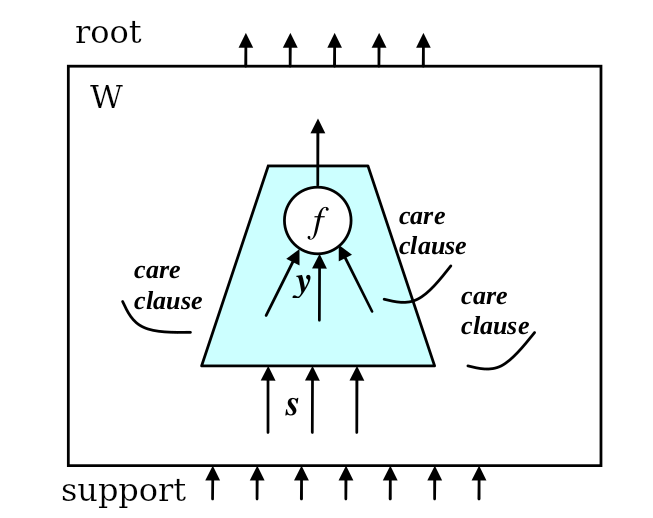
\includegraphics[height=6.5cm]{./windows.png}
\end{center}

\subsubsection{Find Divisor Candidates}
Collect \textit{divisors} from node $f$ to PIs,
avoid these nodes:
\begin{itemize}
    \item the node $f$ itself;
    \item the nodes in the MFFC of $f$.
\end{itemize}
Explore the fanouts of already collected \textit{divisors},
and add the fanouts into \textit{divisors} excepted for:
\begin{itemize}
    \item a divisor has too many fanouts;
    \item nodes in the TFO or in the MFFC of node $f$;
    \item PO nodes;
    \item nodes with large level;
    \item nodes whose fanins are not divisors (I am not clear here);
\end{itemize}

\subsubsection{Construct AIG for Window $W$}
\begin{center}
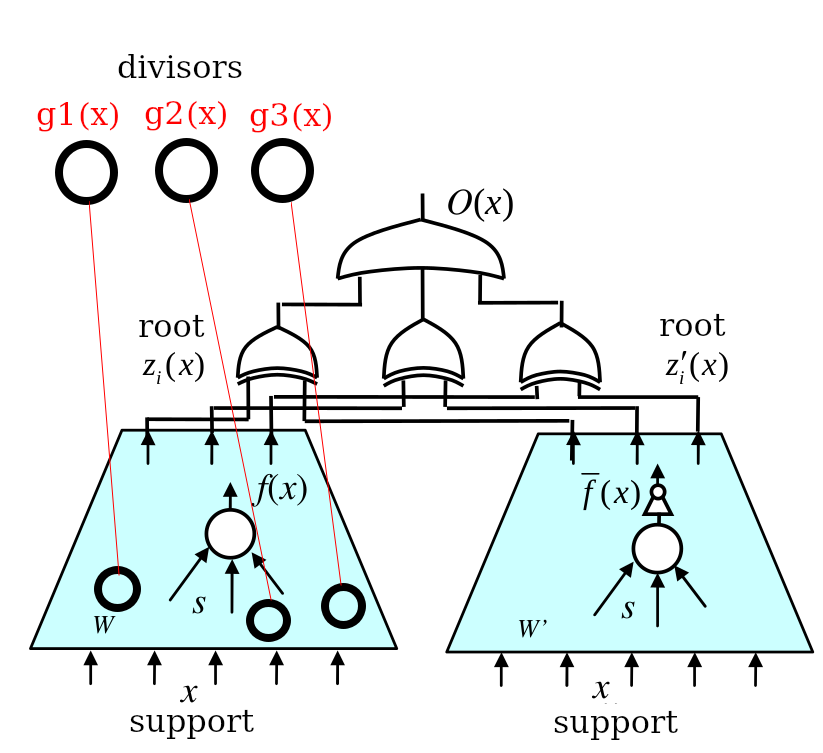
\includegraphics[height=6.5cm]{./aig.png}
\end{center}
If $O(x)$ is asserted to 1,
then $x$ is in the care set of $f$.

\subsubsection{Translate AIG into CNF}

\subsubsection{Create the SAT Problem}
\begin{center}
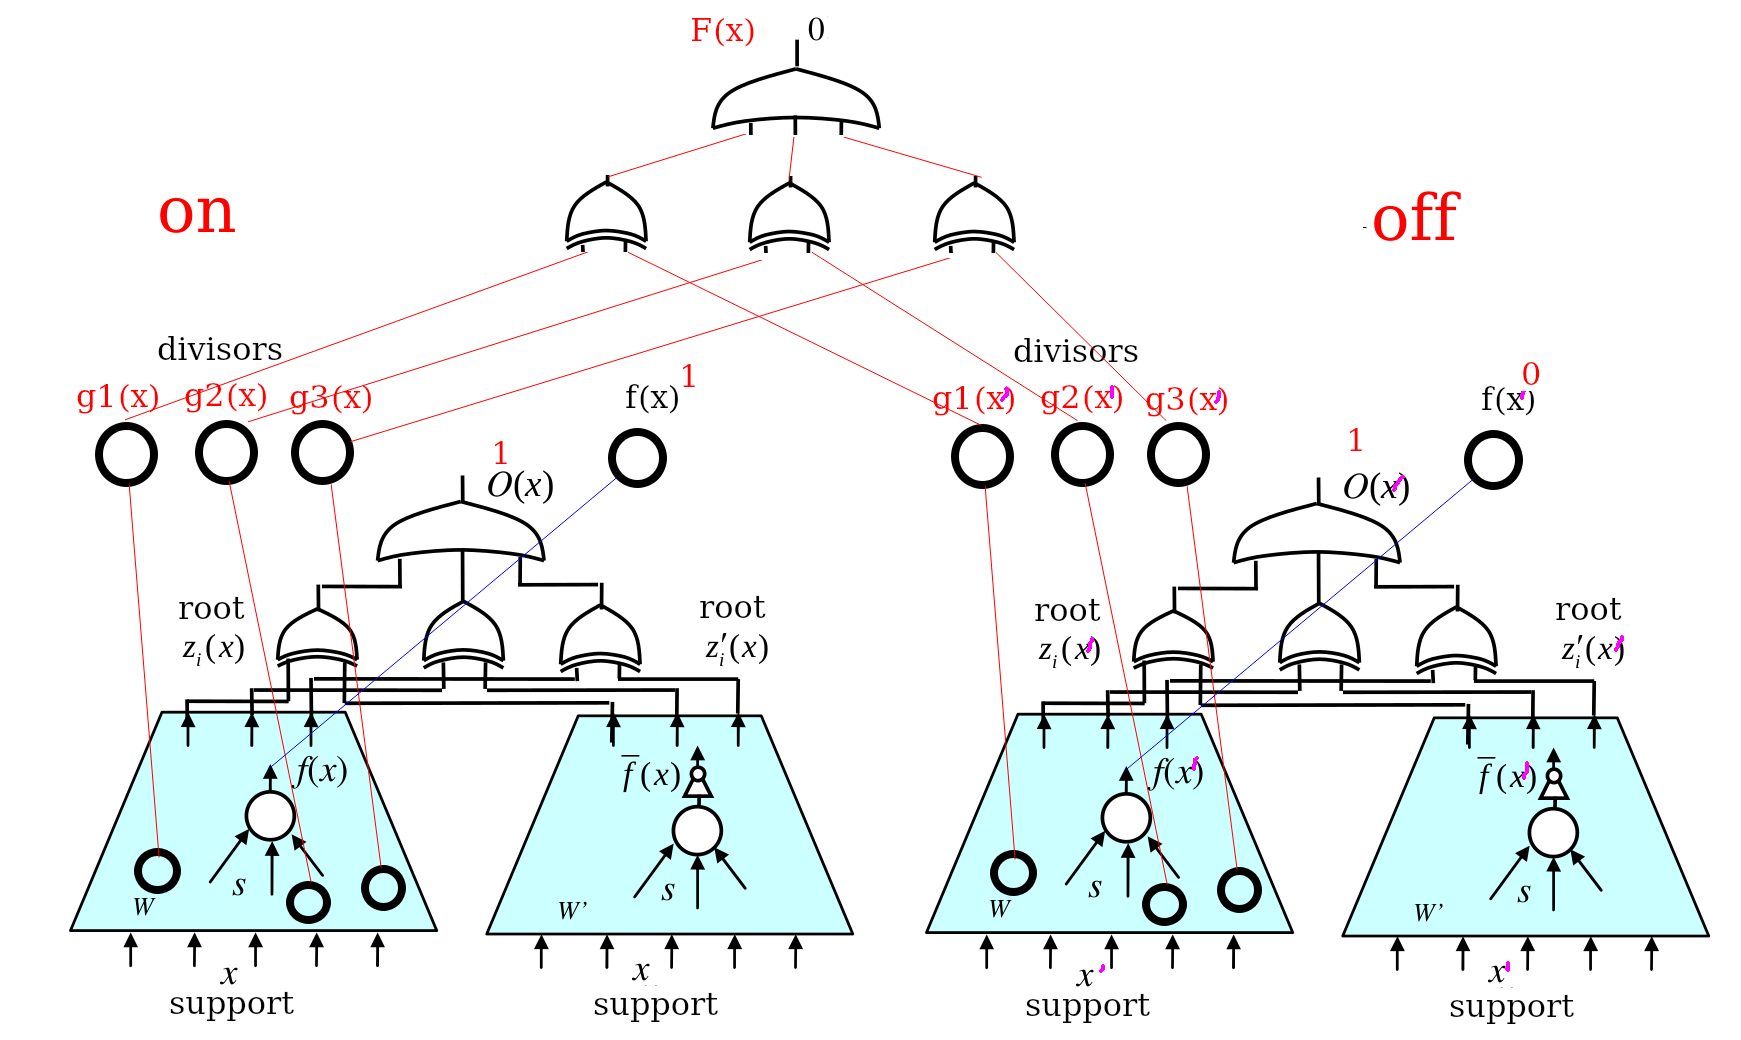
\includegraphics[height=6.5cm]{./sat.png}
\end{center}
Here,
$x$ and $x^\prime$ are different input patterns.
$O(x)$ and $O(x^\prime)$ is asserted to 1,
then $x$ and $x^\prime$ are in $f$'s care set.

\noindent We want to substitute $f = f(s)$ by $f = h(g_1, g_2, \dots, g_n)$.
The dependency function $h$ exists if and only if there is no minterm pair $(x, x^\prime)$,
where $f(x) \neq f(x^\prime)$ and $g_j(x) = g_j(x^\prime)$ for all $j$.
So we assert $f(x) = 1$, $f(x^\prime) = 0$,
all $g_j(x) \oplus g_j(x^\prime) = 0$.

\noindent The CNF expression of the SAT problem is:
\[G = C^{on} f^{on} O^{on} C^{off} \bar f^{off} O^{off} (g_1^{on} \equiv g_1^{off}) \dots (g_n^{on} \equiv g_n^{off})\]

\subsubsection{Interpolation}
To compute a function $h(g)$,
$G$ divided into subsets $A$ and $B$.
\[
    A = C^{on} f^{on} O^{on},
    B = C^{off} \bar f^{off} O^{off} (g_1^{on} \equiv g_1^{off}) \dots (g_n^{on} \equiv g_n^{off})
\]
For unsatisfiable $G$,
the resultant interpolant $A^{\#}$ derived from a refutation proof yields a desired dependency function $h$ (I am not clear here).

Definition of interpolation:
\begin{center}
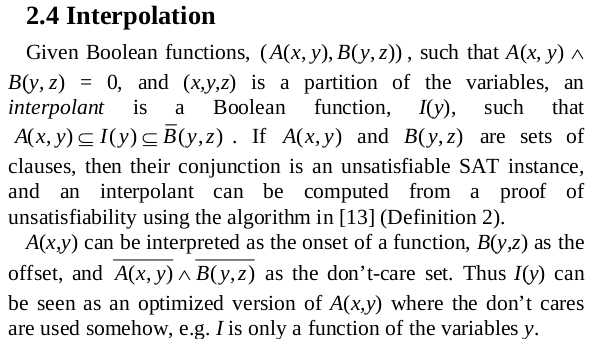
\includegraphics[height=6.5cm]{./interpolation.png}
\end{center}


\subsection{Approximate Version of MFS}
I have no mature idea up to now.

\end{document}
